\tightsection{GO Overview and Challenges}

\comment{
\begin{packeditemize}
	\item System overview.
	\item Workflow of GO backend -- grouping, simplest form
	\item Limitations
\end{packeditemize}
}

\myparasum{Motivated by last section, we have built a real system} The trace-driven preliminary analysis in last section has shown that sharing client-side measurement to predict quality of a new session is feasible. Motivated by these results, we have implemented a working prototype called Video Global Optimization (GO) to realize the goal of accurately predicting the outcome of each decision by sharing measured quality samples from other clients in a {\it centralized} backend, and making best decisions for each session based on the prediction in order to actually improve video quality in the wild.

\myparasum{Organization of this section} This section begins with a design overview of GO. We also introduce the basic workflow of quality prediction and decision making in GO, and highlight the challenges faced by quality prediction algorithms. 


\tightsubsection{GO overview}

\comment{
\begin{packeditemize}
	\item Highlevel components
	\item Quality prediction workflow
\end{packeditemize}
}

\begin{figure}[h!]
\centering
 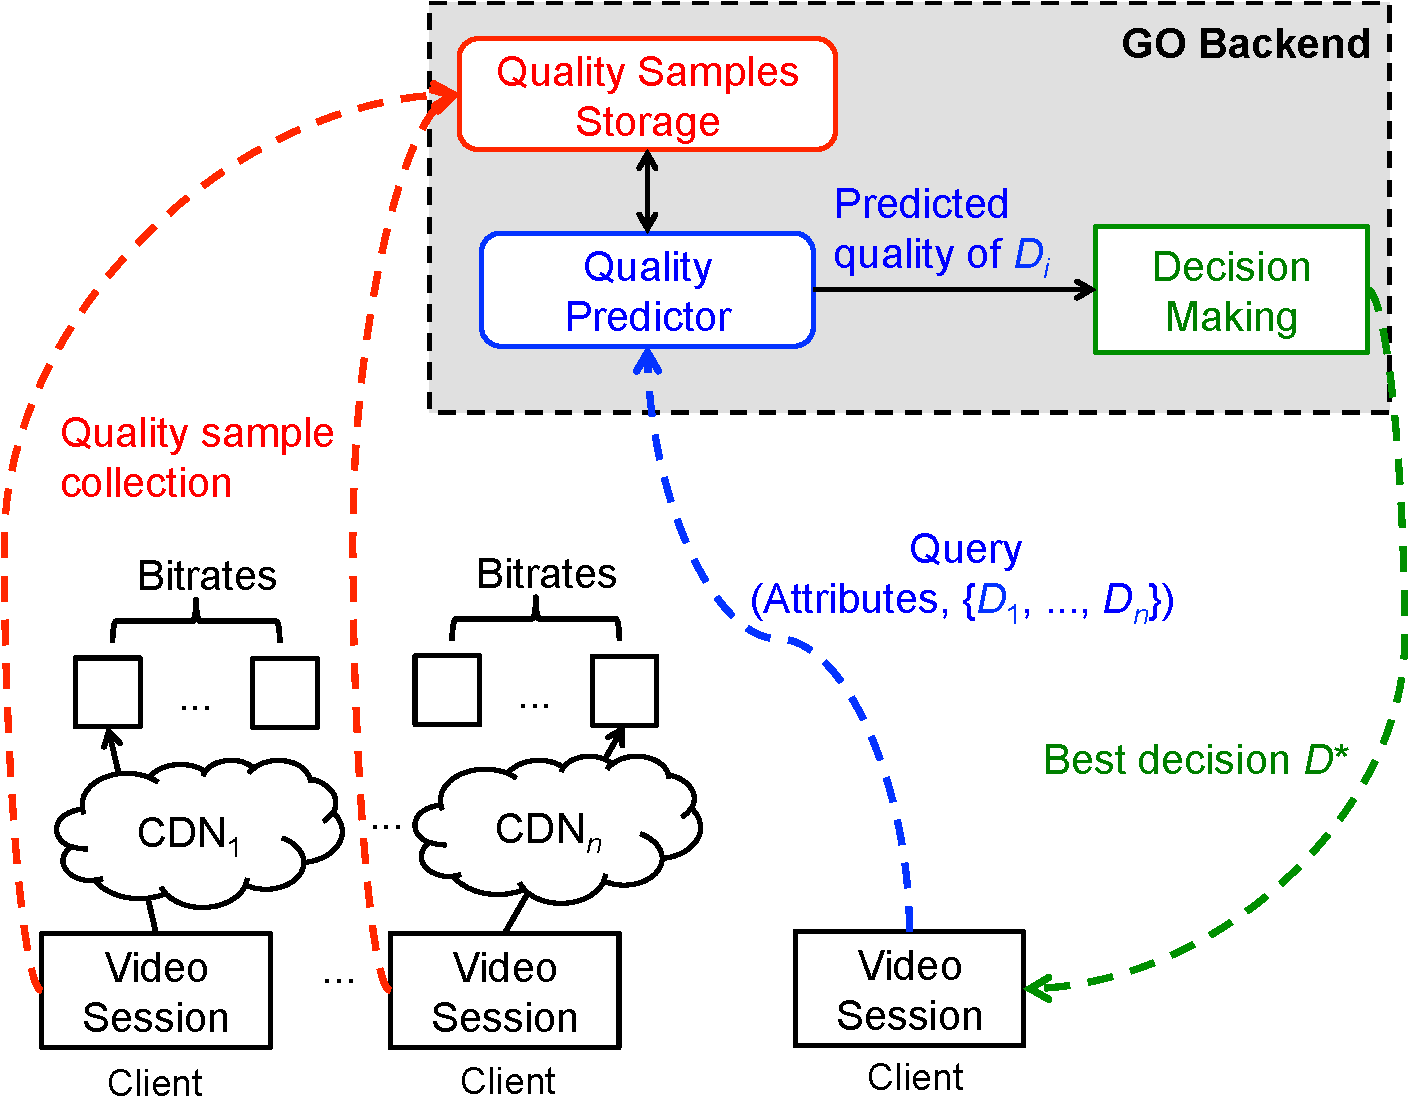
\includegraphics[width=0.5\textwidth] {figures/go-overview.pdf}
\tightcaption{Architecture of GO.}
\label{fig:go-overview}
\end{figure}

\myparasum{Highlevel components} Physically, in order to collect statistics from client and make decision in a centralized manner, GO has two parts: intrumentation code running within players during the cause of a video session at client-side, and GO backend running in publicly available clusters for centralized processing. Logically, there are three components of GO system (see Figure~\ref{fig:go-overview}). 

\myparatight{Quality sample collection} To collect feedback from client-side video sessions, the instrumentation code monitors the state of player and network condition, summarizes them in the form of quality samples (see details in \Section~\ref{subsec:dataset}) and send the quality samples back to GO backend for storage. Quality samples are then stored in a Hadoop File System for storage. \jc{in reality, the raw input from client is in a more raw format of heartbeat. we may decide whether to expose this complexity in scalability section.}

\myparatight{Quality prediction} 

\myparatight{Decision making}




\tightsection{Video Quality Prediction Algorithms}
